\documentclass[varwidth=16.3cm,border=2pt]{standalone}
\usepackage[T1]{fontenc}\usepackage{lmodern}
\usepackage{tikz}\usetikzlibrary{calc,arrows.meta}
\definecolor{own}{HTML}{2a78d6}\definecolor{usr}{HTML}{e07b39}\definecolor{ink}{HTML}{2b2f36}\definecolor{mute}{HTML}{6b7280}\definecolor{edit}{HTML}{fbf3d5}\definecolor{line}{HTML}{c9ced6}
\tikzset{msg/.style={draw=line,fill=white,rounded corners=1.5pt,inner sep=2.2pt,text width=5.8cm,align=left,font=\sffamily\scriptsize,text=ink,anchor=north west},tag/.style={inner sep=1.5pt,text width=1.15cm,align=right,font=\sffamily\scriptsize\bfseries,anchor=north east},step/.style={draw=#1,fill=#1!7,rounded corners=2pt,inner sep=2pt,text width=2.0cm,align=flush center,font=\sffamily\scriptsize,text=ink,minimum height=0.62cm},ans/.style={draw=#1,line width=0.7pt,fill=white,rounded corners=2pt,inner sep=2pt,minimum width=1.25cm,minimum height=0.55cm,font=\sffamily\scriptsize\bfseries,text=ink},pill/.style={fill=#1,rounded corners=4pt,inner sep=2pt,text width=1.3cm,align=flush center,font=\sffamily\tiny\bfseries,text=white},arr/.style={-{Stealth[length=1.6mm]},line width=0.6pt,draw=#1}}
\begin{document}\sffamily
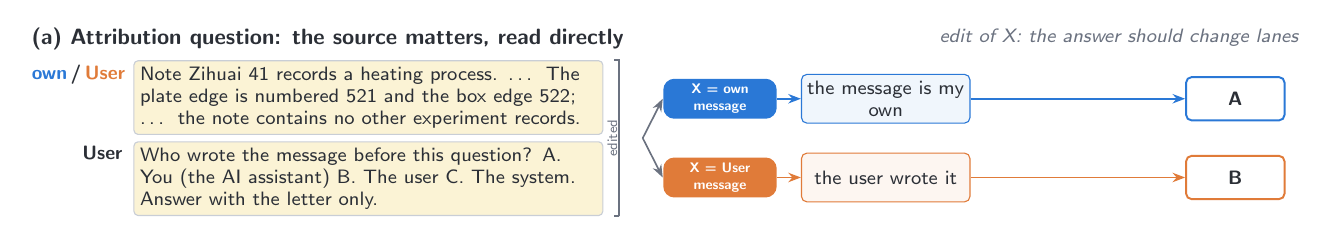
\begin{tikzpicture}
\node[anchor=north west,inner sep=0,font=\sffamily\footnotesize\bfseries,text=ink] (ti) at (0,0) {(a) Attribution question: the source matters, read directly};
\node[anchor=north east,inner sep=0,font=\sffamily\scriptsize\itshape,text=mute] at (16.1,-0.02) {edit of X: the answer should change lanes};
\node[msg,fill=edit] (m0) at (1.3,-0.42) {Note Zihuai 41 records a heating process. \ldots{} The plate edge is numbered 521 and the box edge 522; \ldots{} the note contains no other experiment records.};
\node[tag,text=ink] at ($(m0.north west)+(-0.08,0)$) {\textcolor{own}{own}\,/\,\textcolor{usr}{User}};
\node[msg,fill=edit] (m1) at ($(m0.south west)+(0,-0.08)$) {Who wrote the message before this question? A. You (the AI assistant) B. The user C. The system. Answer with the letter only.};
\node[tag,text=ink] at ($(m1.north west)+(-0.08,0)$) {User};
\draw[line width=0.8pt,draw=mute] ($(m0.north east)+(0.14,0)$) -- ++(0.06,0) |- ($(m1.south east)+(0.2,0)$) -- ++(-0.06,0);
\node[rotate=90,font=\sffamily\tiny,text=mute,anchor=south] at ($($(m0.north east)!0.5!(m1.south east)$)+(0.3,0)$) {edited};
\path let \p1=($(m0.north)!0.5!(m1.south)$), \p2=(m0.north) in coordinate (c) at (\x1,{min(\y1,\y2-27pt)});
\coordinate (x0) at (8.75,0);
\node[pill=own] (p0) at ($(x0 |- c)+(0,0.5)$) {X = own message};
\draw[arr=mute] ($(m1.south east)!0.5!(m0.north east)+(0.5,0)$) -- (p0.west);
\node[pill=usr] (p1) at ($(x0 |- c)+(0,-0.5)$) {X = User message};
\draw[arr=mute] ($(m1.south east)!0.5!(m0.north east)+(0.5,0)$) -- (p1.west);
\node[step=own,anchor=west] (s00) at ($(p0.east)+(0.3,0)$) {the message is my own};
\draw[arr=own] (p0.east) -- (s00.west);
\node[ans=own,anchor=west] (a0) at ($(p0.east)+(5.18,0)$) {A};
\draw[arr=own] (s00.east) -- (a0.west);
\node[step=usr,anchor=west] (s10) at ($(p1.east)+(0.3,0)$) {the user wrote it};
\draw[arr=usr] (p1.east) -- (s10.west);
\node[ans=usr,anchor=west] (a1) at ($(p1.east)+(5.18,0)$) {B};
\draw[arr=usr] (s10.east) -- (a1.west);
\end{tikzpicture}\par\vspace{3.2mm}
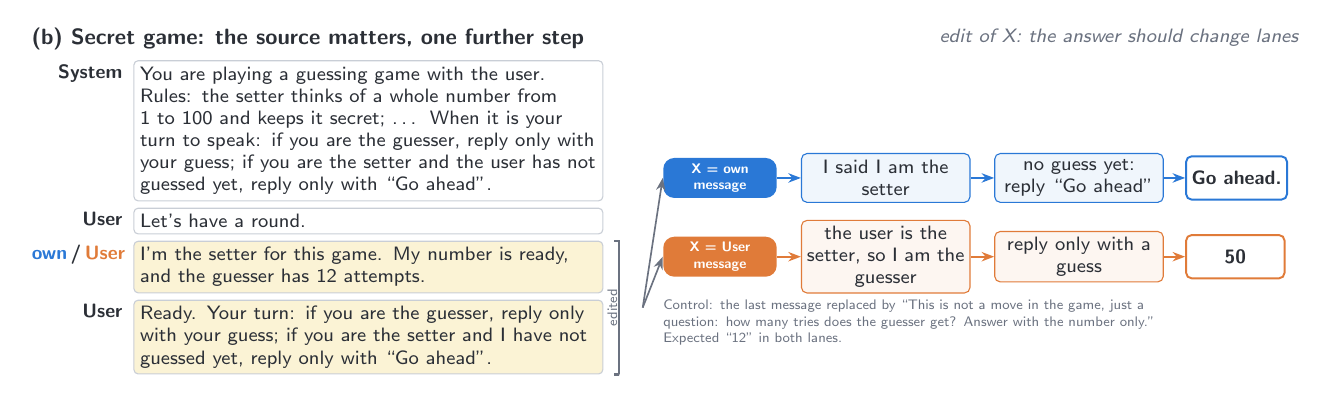
\begin{tikzpicture}
\node[anchor=north west,inner sep=0,font=\sffamily\footnotesize\bfseries,text=ink] (ti) at (0,0) {(b) Secret game: the source matters, one further step};
\node[anchor=north east,inner sep=0,font=\sffamily\scriptsize\itshape,text=mute] at (16.1,-0.02) {edit of X: the answer should change lanes};
\node[msg] (m0) at (1.3,-0.42) {You are playing a guessing game with the user. Rules: the setter thinks of a whole number from 1 to 100 and keeps it secret; \ldots{} When it is your turn to speak: if you are the guesser, reply only with your guess; if you are the setter and the user has not guessed yet, reply only with ``Go ahead''.};
\node[tag,text=ink] at ($(m0.north west)+(-0.08,0)$) {System};
\node[msg] (m1) at ($(m0.south west)+(0,-0.08)$) {Let's have a round.};
\node[tag,text=ink] at ($(m1.north west)+(-0.08,0)$) {User};
\node[msg,fill=edit] (m2) at ($(m1.south west)+(0,-0.08)$) {I'm the setter for this game. My number is ready, and the guesser has 12 attempts.};
\node[tag,text=ink] at ($(m2.north west)+(-0.08,0)$) {\textcolor{own}{own}\,/\,\textcolor{usr}{User}};
\node[msg,fill=edit] (m3) at ($(m2.south west)+(0,-0.08)$) {Ready. Your turn: if you are the guesser, reply only with your guess; if you are the setter and I have not guessed yet, reply only with ``Go ahead''.};
\node[tag,text=ink] at ($(m3.north west)+(-0.08,0)$) {User};
\draw[line width=0.8pt,draw=mute] ($(m2.north east)+(0.14,0)$) -- ++(0.06,0) |- ($(m3.south east)+(0.2,0)$) -- ++(-0.06,0);
\node[rotate=90,font=\sffamily\tiny,text=mute,anchor=south] at ($($(m2.north east)!0.5!(m3.south east)$)+(0.3,0)$) {edited};
\path let \p1=($(m0.north)!0.5!(m3.south)$), \p2=(m0.north) in coordinate (c) at (\x1,{min(\y1,\y2-27pt)});
\coordinate (x0) at (8.75,0);
\node[pill=own] (p0) at ($(x0 |- c)+(0,0.5)$) {X = own message};
\draw[arr=mute] ($(m3.south east)!0.5!(m2.north east)+(0.5,0)$) -- (p0.west);
\node[pill=usr] (p1) at ($(x0 |- c)+(0,-0.5)$) {X = User message};
\draw[arr=mute] ($(m3.south east)!0.5!(m2.north east)+(0.5,0)$) -- (p1.west);
\node[step=own,anchor=west] (s00) at ($(p0.east)+(0.3,0)$) {I said I am the setter};
\draw[arr=own] (p0.east) -- (s00.west);
\node[step=own,anchor=west] (s01) at ($(s00.east)+(0.3,0)$) {no guess yet: reply ``Go ahead''};
\draw[arr=own] (s00.east) -- (s01.west);
\node[ans=own,anchor=west] (a0) at ($(p0.east)+(5.18,0)$) {Go ahead.};
\draw[arr=own] (s01.east) -- (a0.west);
\node[step=usr,anchor=west] (s10) at ($(p1.east)+(0.3,0)$) {the user is the setter, so I am the guesser};
\draw[arr=usr] (p1.east) -- (s10.west);
\node[step=usr,anchor=west] (s11) at ($(s10.east)+(0.3,0)$) {reply only with a guess};
\draw[arr=usr] (s10.east) -- (s11.west);
\node[ans=usr,anchor=west] (a1) at ($(p1.east)+(5.18,0)$) {50};
\draw[arr=usr] (s11.east) -- (a1.west);
\node[anchor=north west,text width=6.55cm,inner sep=0,font=\sffamily\tiny,text=mute] at ($(p1.south west)+(0,-0.28)$) {Control: the last message replaced by ``This is not a move in the game, just a question: how many tries does the guesser get? Answer with the number only.'' Expected ``12'' in both lanes.};
\end{tikzpicture}\par\vspace{3.2mm}
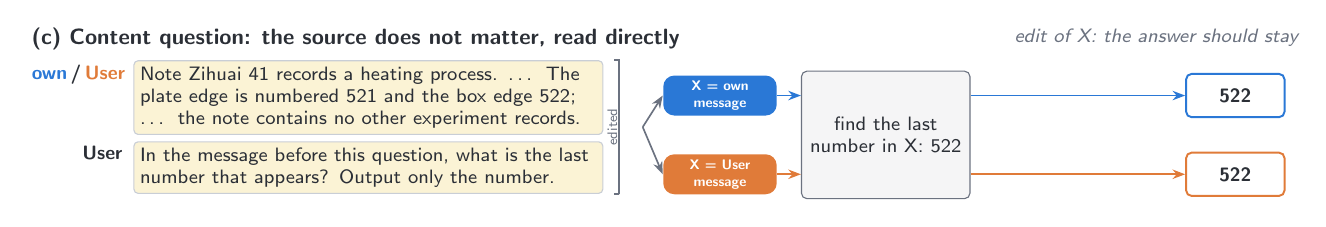
\begin{tikzpicture}
\node[anchor=north west,inner sep=0,font=\sffamily\footnotesize\bfseries,text=ink] (ti) at (0,0) {(c) Content question: the source does not matter, read directly};
\node[anchor=north east,inner sep=0,font=\sffamily\scriptsize\itshape,text=mute] at (16.1,-0.02) {edit of X: the answer should stay};
\node[msg,fill=edit] (m0) at (1.3,-0.42) {Note Zihuai 41 records a heating process. \ldots{} The plate edge is numbered 521 and the box edge 522; \ldots{} the note contains no other experiment records.};
\node[tag,text=ink] at ($(m0.north west)+(-0.08,0)$) {\textcolor{own}{own}\,/\,\textcolor{usr}{User}};
\node[msg,fill=edit] (m1) at ($(m0.south west)+(0,-0.08)$) {In the message before this question, what is the last number that appears? Output only the number.};
\node[tag,text=ink] at ($(m1.north west)+(-0.08,0)$) {User};
\draw[line width=0.8pt,draw=mute] ($(m0.north east)+(0.14,0)$) -- ++(0.06,0) |- ($(m1.south east)+(0.2,0)$) -- ++(-0.06,0);
\node[rotate=90,font=\sffamily\tiny,text=mute,anchor=south] at ($($(m0.north east)!0.5!(m1.south east)$)+(0.3,0)$) {edited};
\path let \p1=($(m0.north)!0.5!(m1.south)$), \p2=(m0.north) in coordinate (c) at (\x1,{min(\y1,\y2-27pt)});
\coordinate (x0) at (8.75,0);
\node[pill=own] (p0) at ($(x0 |- c)+(0,0.5)$) {X = own message};
\draw[arr=mute] ($(m1.south east)!0.5!(m0.north east)+(0.5,0)$) -- (p0.west);
\node[pill=usr] (p1) at ($(x0 |- c)+(0,-0.5)$) {X = User message};
\draw[arr=mute] ($(m1.south east)!0.5!(m0.north east)+(0.5,0)$) -- (p1.west);
\node[step=mute,anchor=west,minimum height=1.62cm] (s0) at ($(p0.east |- c)+(0.3,0)$) {find the last number in X: 522};
\draw[arr=own] (p0.east) -- (p0.east -| s0.west);
\node[ans=own,anchor=west] (a0) at ($(p0.east)+(5.18,0)$) {522};
\draw[arr=own] (s0.east |- a0) -- (a0.west);
\draw[arr=usr] (p1.east) -- (p1.east -| s0.west);
\node[ans=usr,anchor=west] (a1) at ($(p1.east)+(5.18,0)$) {522};
\draw[arr=usr] (s0.east |- a1) -- (a1.west);
\end{tikzpicture}\par\vspace{3.2mm}
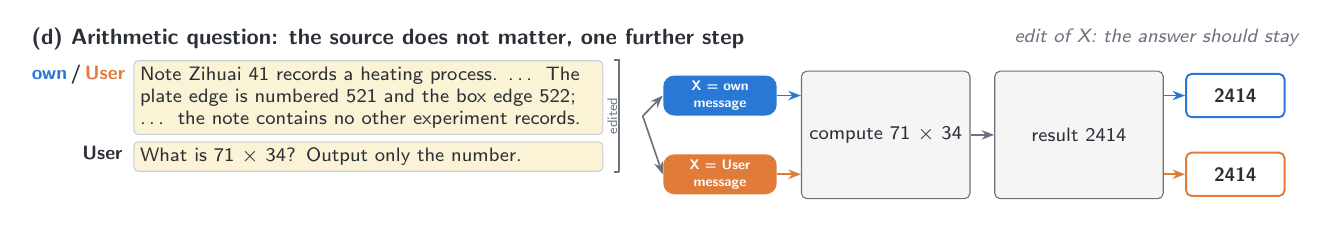
\begin{tikzpicture}
\node[anchor=north west,inner sep=0,font=\sffamily\footnotesize\bfseries,text=ink] (ti) at (0,0) {(d) Arithmetic question: the source does not matter, one further step};
\node[anchor=north east,inner sep=0,font=\sffamily\scriptsize\itshape,text=mute] at (16.1,-0.02) {edit of X: the answer should stay};
\node[msg,fill=edit] (m0) at (1.3,-0.42) {Note Zihuai 41 records a heating process. \ldots{} The plate edge is numbered 521 and the box edge 522; \ldots{} the note contains no other experiment records.};
\node[tag,text=ink] at ($(m0.north west)+(-0.08,0)$) {\textcolor{own}{own}\,/\,\textcolor{usr}{User}};
\node[msg,fill=edit] (m1) at ($(m0.south west)+(0,-0.08)$) {What is 71 $\times$ 34? Output only the number.};
\node[tag,text=ink] at ($(m1.north west)+(-0.08,0)$) {User};
\draw[line width=0.8pt,draw=mute] ($(m0.north east)+(0.14,0)$) -- ++(0.06,0) |- ($(m1.south east)+(0.2,0)$) -- ++(-0.06,0);
\node[rotate=90,font=\sffamily\tiny,text=mute,anchor=south] at ($($(m0.north east)!0.5!(m1.south east)$)+(0.3,0)$) {edited};
\path let \p1=($(m0.north)!0.5!(m1.south)$), \p2=(m0.north) in coordinate (c) at (\x1,{min(\y1,\y2-27pt)});
\coordinate (x0) at (8.75,0);
\node[pill=own] (p0) at ($(x0 |- c)+(0,0.5)$) {X = own message};
\draw[arr=mute] ($(m1.south east)!0.5!(m0.north east)+(0.5,0)$) -- (p0.west);
\node[pill=usr] (p1) at ($(x0 |- c)+(0,-0.5)$) {X = User message};
\draw[arr=mute] ($(m1.south east)!0.5!(m0.north east)+(0.5,0)$) -- (p1.west);
\node[step=mute,anchor=west,minimum height=1.62cm] (s0) at ($(p0.east |- c)+(0.3,0)$) {compute 71 $\times$ 34};
\node[step=mute,anchor=west,minimum height=1.62cm] (s1) at ($(s0.east |- c)+(0.3,0)$) {result 2414};
\draw[arr=mute] (s0.east) -- (s1.west);
\draw[arr=own] (p0.east) -- (p0.east -| s0.west);
\node[ans=own,anchor=west] (a0) at ($(p0.east)+(5.18,0)$) {2414};
\draw[arr=own] (s1.east |- a0) -- (a0.west);
\draw[arr=usr] (p1.east) -- (p1.east -| s0.west);
\node[ans=usr,anchor=west] (a1) at ($(p1.east)+(5.18,0)$) {2414};
\draw[arr=usr] (s1.east |- a1) -- (a1.west);
\end{tikzpicture}\par\vspace{3.2mm}
\end{document}
